\documentclass[border=3mm]{standalone}

\usepackage{tikz}
\usetikzlibrary{3d,arrows.meta,angles}

\begin{document}
	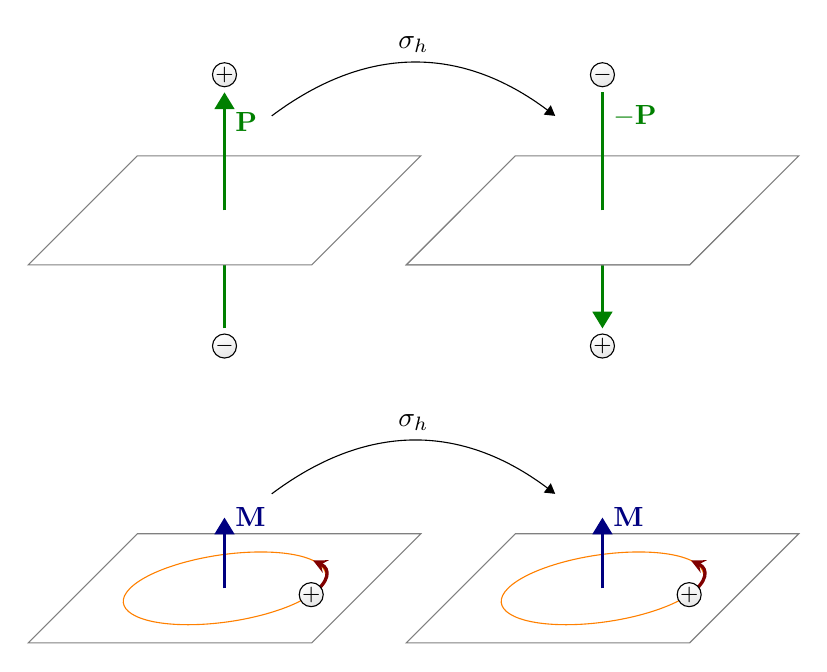
\begin{tikzpicture}[scale=1.2]
	
		\tikzstyle{charge+}=[draw,circle,inner sep=0pt,outer sep=2pt,thin,top color=white!50,bottom color=white!90!black,shading angle=20]
		\tikzstyle{charge-}=[draw,circle,inner sep=0pt,outer sep=2pt,thin,top color=white!50,bottom color=white!90!black,shading angle=20]
		%% Top left
		\begin{scope}
			\begin{scope}[canvas is zy plane at x=0]
				\draw[very thick,green!50!black] (0,-1.25) coordinate (a) -- (0,0);
				\node[charge-,below] at (a) {\footnotesize $-$};
			\end{scope}
			\begin{scope}[canvas is xz plane at y=0]
				\draw[gray,fill=white] (1.5,-1.5) rectangle(-1.5,1.5);
			\end{scope}
			\begin{scope}[canvas is zy plane at x=0]
				\draw[very thick,green!50!black,-Triangle] (0,0) -- (0,1.25) coordinate (b) node[pos=0.75,right]{$\mathbf{P}$};
				\node[charge+,above] at (b) {\footnotesize $+$};
			\end{scope}
				\draw[-Triangle] (0.5,1) .. controls (1.5,1.75) and (2.5,1.75) .. (3.5,1) node[above,midway]{$\sigma_{h}$};
		\end{scope}
		
		%% Top right
		\begin{scope}[xshift=4cm]
			\begin{scope}[canvas is zy plane at x=0]
				\draw[very thick,green!50!black,Triangle-] (0,-1.25) coordinate (a) -- (0,0);
				\node[charge+,below] at (a) {\footnotesize $+$};
			\end{scope}
			\begin{scope}[canvas is xz plane at y=0]
				\draw[gray,fill=white] (1.5,-1.5) rectangle(-1.5,1.5);
			\end{scope}
			\begin{scope}[canvas is zy plane at x=0]
				\draw[very thick,green!50!black] (0,0) -- (0,1.25) coordinate (b) node[pos=0.8,right]{$\mathbf{-P}$};
				\node[charge-,above] at (b) {\footnotesize $-$};
			\end{scope}
			\begin{scope}[canvas is xz plane at y=0]
				\draw[gray] (1.5,0) -- (1.5,1.5) -- (-1.5,1.5) -- (-1.5,0);
			\end{scope}
		\end{scope}
		
		\begin{scope}[yshift=-4cm]
			
			%% Bottom left
			\begin{scope}[canvas is xz plane at y=0]
				\draw[gray] (1.5,1.5) rectangle (-1.5,-1.5);
			\end{scope}
			\begin{scope}[canvas is xz plane at y=0]
				\draw[orange] (0,0) circle (1);
				\coordinate (d) at (10:1);
				\draw[red!50!black,-stealth,very thick] (d) arc (10:-50:1);
				\node[charge+] at (d) {\footnotesize $+$};
			\end{scope}
			\begin{scope}[canvas is zy plane at x=0]
				\draw[very thick,blue!50!black,-Triangle] (0,0) -- (0,0.75) node[right] {$\mathbf{M}$};
			\end{scope}
			\draw[-Triangle] (0.5,1) .. controls (1.5,1.75) and (2.5,1.75) .. (3.5,1) node[above,midway]{$\sigma_{h}$};
		\end{scope}
		
			%% Bottom right
		\begin{scope}[yshift=-4cm,xshift=4cm]
			\begin{scope}[canvas is xz plane at y=0]
				\draw[gray] (1.5,1.5) rectangle (-1.5,-1.5);
			\end{scope}
			\begin{scope}[canvas is xz plane at y=0]
				\draw[orange] (0,0) circle (1);
				\coordinate (d) at (10:1);
				\draw[red!50!black,-stealth,very thick] (d) arc (10:-50:1);
				\node[charge+] at (d) {\footnotesize $+$};
			\end{scope}
			\begin{scope}[canvas is zy plane at x=0]
				\draw[very thick,blue!50!black,-Triangle] (0,0) -- (0,0.75) node[right] {$\mathbf{M}$};
			\end{scope}
			
		\end{scope}
	\end{tikzpicture}
\end{document}
